% TODO: what to put here?
In this section we summarize the results of the experiments described in Section~\ref{s:exp}.
% In this section we summarize the results of the experiments examining
% the influence of risk group dynamics on simulated epidemics.
% The aim of the experiments was to explore the impact of
% different implementations of risk group dynamics on model outputs
% in a generalized epidemic model.
% We compare the projected incidence and prevalence across
% four model variants and range of turnover magnitudes,
% as well as the estimated TPAF of the high risk group, with and without turnover.
% ==================================================================================================
\subsection{Model Variants}\label{ss:res-variants}
First, the comparisons of models with and without
key features of risk group dynamics are presented.
% --------------------------------------------------------------------------------------------------
\paragraph{Experiment 1.1: Heterogeneity in Risk}\label{p:res-1-hetero}
Figure~\ref{fig:compare-hetero-prevalence} shows the modelled prevalence
with and without heterogeneity in risk (Full~vs~V1).
As previously noted in discussions of core group theory~\citep{Yorke1978,Stigum1994},
epidemic dynamics and endemic equilibrium are influenced by the presence of
heterogeneity in risk within a population.
For this model and parameters (Table~\ref{tab:params-base}),
failure to model heterogeneity in risk (V1) results in
a basic reproduction number $R_0 < 1$, and no epidemic,
while the model with heterogeneity (Full) predicts a nonzero endemic equilibrium.
%% JK: this result is not always the case,
%% but is it worth dwelling on here, as it is not the focus of the paper?
% --------------------------------------------------------------------------------------------------
\paragraph{Experiment 1.2: Population Growth}\label{p:res-1-growth}
Figure~\ref{fig:compare-growth-prevalence} shows the modelled prevalence
with and without population growth (Full~vs~V2).
Inclusion of population growth in the model
results in lower equilibrium prevalence.
This result can be explained following the results of \citet{Hadeler1990},
who observed that under exponential population growth,
and without disease-attributable mortality,
the rate of growth of susceptible individuals exceeds
the rate of growth of infected individuals.
Thus equilibrium prevalence declines
relative to a model with constant population size.
For a simplified version of the model used here,
the relationship between equilibrium prevalence and model entry rate $\nu$
is also given in \ref{aa:eqs-growth}.
%% JK: I'm not confident in this derivation, but again, not the focus of the paper.
%% can we omit, and simply cite Hadeler1990?
\begin{figure}
  \centering
  \begin{subfigure}{0.45\linewidth}
    \centering
    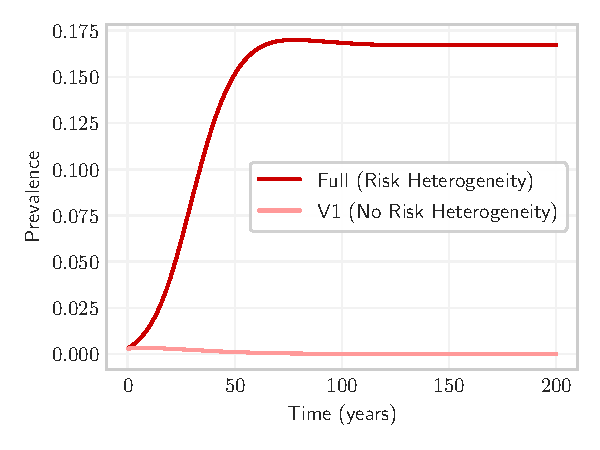
\includegraphics[width=\linewidth]{hetero-prevalence-all}
    \caption{Risk heterogeneity (Full~vs~V1)}
    \label{fig:compare-hetero-prevalence}
  \end{subfigure}
  \begin{subfigure}{0.45\linewidth}
    \centering
    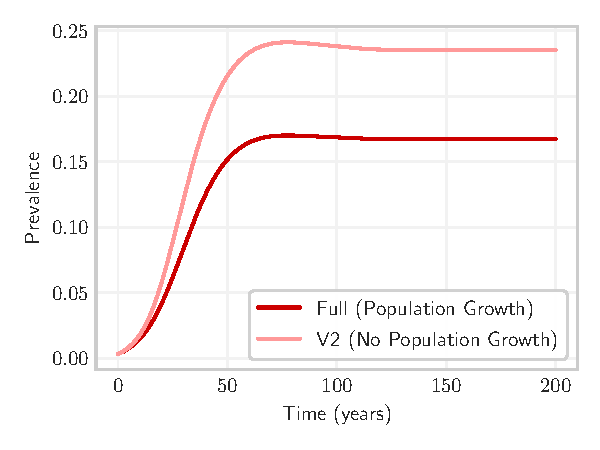
\includegraphics[width=\linewidth]{growth-prevalence-all}
    \caption{Population growth (Full~vs~V2)}
    \label{fig:compare-growth-prevalence}
  \end{subfigure}
  \caption{Comparison of model projections
    with and without risk heterogeneity and
    with and without population growth}
\end{figure}
% --------------------------------------------------------------------------------------------------
\paragraph{Experiment 1.3: Turnover}\label{p:res-1-turnover}
Finally, the influence of including risk group turnover in an epidemic model
on equilibrium prevalence is considered.
Under the default treatment rate $\tau = 0.1$,
overall projected equilibrium prevalence is slightly higher with turnover than without
(Figure~\ref{fig:compare-turnover-prevalence-all-tau=0.1}).
However, if the treatment rate is increased to $\tau = 0.2$,
the model with turnover projects
a lower equilibrium prevalence than the model without turnover
(Figure~\ref{fig:compare-turnover-prevalence-all-tau=0.2}).
Thus, inclusion of risk group turnover influences the equilibrium prevalence.
The nature of this influence, however, depends on several factors,
including treatment rate and risk group parameters.
The next section aims to clarify and explain this influence
through exploration of group-specific incidence and prevalence at equilibrium
under different rates of turnover $\phi$ and treatment $\tau$.
\begin{figure}
  \centering
  \begin{subfigure}{0.45\linewidth}
    \centering
    \includegraphics[width=\linewidth]{{turnover-prevalence-all-tau=0.1}.pdf}
    \caption{Treatment rate $\tau= 0.2$}
    \label{fig:compare-turnover-prevalence-all-tau=0.1}
  \end{subfigure}
  \begin{subfigure}{0.45\linewidth}
    \centering
    \includegraphics[width=\linewidth]{{turnover-prevalence-all-tau=0.2}.pdf}
    \caption{Treatment rate $\tau= 0.2$}
    \label{fig:compare-turnover-prevalence-all-tau=0.2}
  \end{subfigure}
  \caption{Comparison of overall projected prevalence with and without risk group turnover
    (Full~vs~V3 model variants),
    under two different treatment rates $\tau$.}
  \label{fig:compare-turnover-prevalence}
\end{figure}
% ==================================================================================================
\subsection{Influence of Turnover}\label{ss:res-turnover}
This section presents trends in the influence turnover
on incidence and prevalence for epidemic systems at equilibrium.
% --------------------------------------------------------------------------------------------------
\paragraph{Experiment 2.1: Turnover Magnitude}
Figure~\ref{fig:1d-prevalence} illustrates trends in equilibrium prevalence versus turnover
among the high and low risk groups, as well as overall.
As turnover increases, prevalence among the highest risk group decreases
(Figure~\ref{fig:1d-prevalence-high}).
This is because
the proportion of individuals exiting the highest risk group via turnover who are infected
is higher than
the proportion of individuals entering the highest risk group via turnover who are infected,
since prevalence is highest in the highest risk group.
That is, the highest risk group experiences a net reduction in the number of infected individuals
(illustrated in Figure~\ref{fig:flows}).
For low to moderate rates of turnover,
this exchange also increases prevalence among the lowest risk group
(Figure~\ref{fig:1d-prevalence-low}, region~A),
and the population overall
(Figure~\ref{fig:1d-prevalence-all}, region~A).%
\footnote{In this model, the lowest risk group usually dominates trends in overall prevalence
  because this risk group represents 75\% of the population
  (Table~\ref{tab:params-base}: $\bm{\hat{x}}$).}
However, at high rates of turnover,
turnover decreases the prevalence among the lowest risk group and overall
(Figure~\ref{fig:1d-prevalence-low}~and~\ref{fig:1d-prevalence-all}, region~B),
This peak and decline is due to the influence of turnover on incidence,
which we have not yet discussed.
\begin{figure}
  \centering
  \begin{subfigure}{0.45\linewidth}
    \centering
    \includegraphics[width=\linewidth]{{1d-prevalence-high-tau=0.1}.pdf}
    \caption{High risk}
    \label{fig:1d-prevalence-high}
  \end{subfigure}
  \begin{subfigure}{0.45\linewidth}
    \centering
    \includegraphics[width=\linewidth]{{1d-prevalence-low-tau=0.1}.pdf}
    \caption{Low risk}
    \label{fig:1d-prevalence-low}
  \end{subfigure}
  \begin{subfigure}{0.45\linewidth}
    \centering
    \includegraphics[width=\linewidth]{{1d-prevalence-all-tau=0.1}.pdf}
    \caption{Overall}
    \label{fig:1d-prevalence-all}
  \end{subfigure}
  \caption{Equilibrium prevalence among risk groups versus turnover,
    as controlled by the duration in the high risk group $\delta_H$.
    Turnover shown in log scale.}
  \label{fig:1d-prevalence}
\end{figure}
\begin{figure}
  \centering
  \begin{subfigure}[t]{0.4\linewidth}
    \centering
    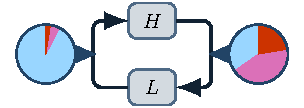
\includegraphics[width=\linewidth]{flows-low.pdf}
    \caption{Low turnover: region~A}
    \label{fig:flows-low}
  \end{subfigure}%
  \begin{subfigure}[t]{0.4\linewidth}
    \centering
    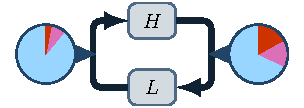
\includegraphics[width=\linewidth]{flows-high.pdf}
    \caption{High turnover: region~B}
    \label{fig:flows-high}
  \end{subfigure}%
  \begin{subfigure}[t]{0.2\linewidth}
    \centering
    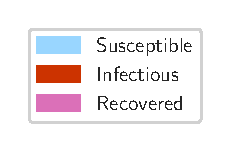
\includegraphics[width=\linewidth]{flows-legend.pdf}
  \end{subfigure}
  \caption{Illustrative schematic showing average health states of individuals
    moving between high and low risk groups due to different rates of turnover.
    Turnover acts to homogenize the distribution of health states across risk groups.}
  \label{fig:flows}
\end{figure}
\par
To understand the influence of turnover on incidence in this model,
consider the force of infection equation, Eq~(\ref{eq:foi}).
As shown in \ref{aa:eqs-incidence}, the driving component in this expression is
the proportion of available partnerships which are offered by infectious individuals,
denoted as $\bm{C}_{\mathcal{I}}$.
This component can be further broken down into the following two factors:
1)~the average contact rate among infectious individuals $\hat{C}_{\mathcal{I}}$, and
2)~the proportion of the population who are infectious $\hat{\mathcal{I}}$.
Thus the influence of turnover on overall incidence
can be understood through the influence of turnover on these two factors.
\par
As shown in Figure~\ref{fig:1d-C-I}, turnover decreases
$\hat{C}_{\mathcal{I}}$ the average contact rate among infectious individuals.
This is because turnover results in a net movement of infected individuals
from high to low risk (Figure~\ref{fig:flows}) \citep{Henry2015}.
However, at low to moderate rates of turnover, turnover increases
$\hat{\mathcal{I}}$ the proportion of the population who are infectious
(Figure~\ref{fig:1d-X-I}, region~A).
This is related to the overall increase in prevalence with turnover
shown in region~A of Figure~\ref{fig:1d-prevalence-all} \citep{Zhang2012}.
Under the conditions shown in region~A of Figure~\ref{fig:1d-incidence-factors},
the proportion of the population who are infectious $\hat{\mathcal{I}}$
increases faster with turnover than
the average contact rate of infectious people $\hat{C}_{\mathcal{I}}$ decreases.
Thus the overall $\bm{C}_{\mathcal{I}}$ increases with turnover in region~A
(Figure~\ref{fig:1d-XC-I})
and incidence increases proportionally
(Figure~\ref{fig:1d-incidence-all}).
\par
It therefore follows that the peak in incidence, and
the transition between regions A~and~B in Figure~\ref{fig:1d-XC-I}
occurs when the dominating factor
between $\hat{\mathcal{I}}$ and $\hat{C}_{\mathcal{I}}$ reverses.
That is, the transition occurs when
the average contact rate of infectious people
$\hat{C}_{\mathcal{I}}$ decreases due to turnover
more than the proportion of the population who are infectious
$\hat{\mathcal{I}}$ increases due to turnover.
As rates of turnover continue to increase,
declining incidence then reverses the upward trend in $\hat{\mathcal{I}}$,
and incidence and prevalence decrease across all groups in a snowball effect.
This mechanism then explains the observations shown in region~B throughout.
\par
Finally, it is worth noting that
the rates of turnover which maximize incidence
(Figure~\ref{fig:1d-incidence-all}) are lower than
the rates of turnover which maximize prevalence
among the lowest risk group, as well as prevalence overall
(Figure~\ref{fig:1d-prevalence-low}~and~\ref{fig:1d-prevalence-all}).
That is, incidence ``peaks'' first with respect to turnover.
This is because, after peak incidence,
increasing turnover may reduce the total number of infections,
but it still moves infected individuals from high to low risk
(Figure~\ref{fig:flows}).
\begin{figure}[h]
  \centering
  \begin{subfigure}{0.45\linewidth}
    \centering
    \includegraphics[width=\linewidth]{{1d-C-I-tau=0.1}.pdf}
    \caption{Average contact rate among infectious individuals $\hat{C}_{\mathcal{I}}$}
    \label{fig:1d-C-I}
  \end{subfigure}
  \begin{subfigure}{0.45\linewidth}
    \centering
    \includegraphics[width=\linewidth]{{1d-X-I-tau=0.1}.pdf}
    \caption{Proportion of the population who are infectious $\hat{\mathcal{I}}$}
    \label{fig:1d-X-I}
  \end{subfigure}
  \begin{subfigure}[t]{0.45\linewidth}
    \centering
    \includegraphics[width=\linewidth]{{1d-XC-I-tau=0.1}.pdf}
    \caption{Proportion of available partnerships
      which are offered by infectious individuals $\bm{C}_{\mathcal{I}}$}
    \label{fig:1d-XC-I}
  \end{subfigure}
  \begin{subfigure}[t]{0.45\linewidth}
    \centering
    \includegraphics[width=\linewidth]{{1d-incidence-all-tau=0.1}.pdf}
    \caption{Overall incidence $\lambda$}
    \label{fig:1d-incidence-all}
  \end{subfigure}
  \caption{Incidence and the dynamic factors of incidence versus turnover.
    The product of components (a) and (b) is proportional to
    (c) the proportion of total available contacts which are with infectious individuals
    and (d) overall incidence.}
  \label{fig:1d-incidence-factors}
\end{figure}
% --------------------------------------------------------------------------------------------------
\paragraph{Experiment 2.2: Turnover and Treatment Rate}
So far, the influence of turnover on equilibrium incidence and prevalence
has been explored for a single treatment rate.
This section explores additional treatment rates $\tau$.
First, the factors of incidence are considered in Figure~\ref{fig:2d-incidence-factors}.
Increasing the treatment rate $\tau$ actually increases
the average contact rate of infectious individuals $\hat{C}_{\mathcal{I}}$
(Figure~\ref{fig:2d-C-I}).
This is because increasing treatment concentrates infections in the highest risk group,
%[\textit{JK: need to find citation!}],
so that $\hat{C}_{\mathcal{I}}$, on average, increases.
However, increasing treatment reduces
the proportion of the population who are infectious $\hat{\mathcal{I}}$
(Figure~\ref{fig:2d-X-I}),
as the rate of transition between $\mathcal{I}$ and $\mathcal{R}$ increases.
The dominant effect is that of $\hat{\mathcal{I}}$,
which tends towards zero faster than $\hat{C}_{\mathcal{I}}$ tends towards infinity.
Thus, incidence declines with treatment
(Figure~\ref{fig:2d-incidence-all}).
\par
Figure~\ref{fig:2d-incidence-all} also shows that
the rate of turnover which maximizes incidence decreases with treatment.
That is, as treatment rates increase,
turnover is more likely to decrease incidence than it is to increase incidence
(region B grows).
This effect can be explained as follows.
Recall that the mechanism by which turnover decreases incidence is through
reduction of the average contact rate of infectious individuals $\hat{C}_{\mathcal{I}}$,
due to net movement of infectious individuals from high to low risk
(Figure~\ref{fig:flows}).
If treatment increases the concentration of infections in the high risk group,
then the average contact rate of infectious individuals $\hat{C}_{\mathcal{I}}$
will be more sensitive to redistribution of those infectious individuals via turnover.
In Figure~\ref{fig:2d-C-I},
this is shown as the larger downward slope of $\hat{C}_{\mathcal{I}}$ versus turnover
at higher treatment rates (darker blue).
Therefore, at higher treatment rates,
turnover is more likely to decrease incidence
because movement of infectious individuals from high to low risk
has a larger impact on the average contact rate of infectious individuals.
\begin{figure}[h]
  \centering
  \begin{subfigure}[t]{0.45\linewidth}
    \centering
    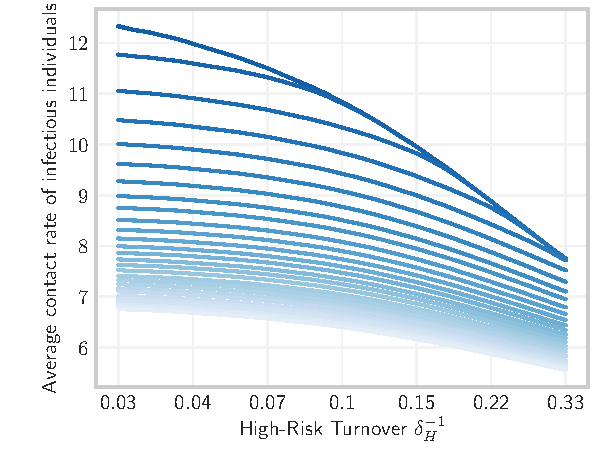
\includegraphics[width=\linewidth]{2d-C-I}
    \caption{Average contact rate among infectious individuals $\hat{C}_{\mathcal{I}}$}
    \label{fig:2d-C-I}
  \end{subfigure}
  \begin{subfigure}[t]{0.45\linewidth}
    \centering
    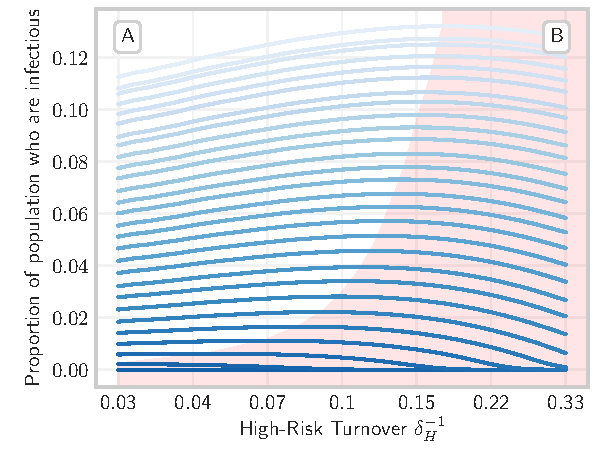
\includegraphics[width=\linewidth]{2d-X-I}
    \caption{Proportion of the population who are infectious $\hat{\mathcal{I}}$}
    \label{fig:2d-X-I}
  \end{subfigure}
  \begin{subfigure}[t]{0.45\linewidth}
    \centering
    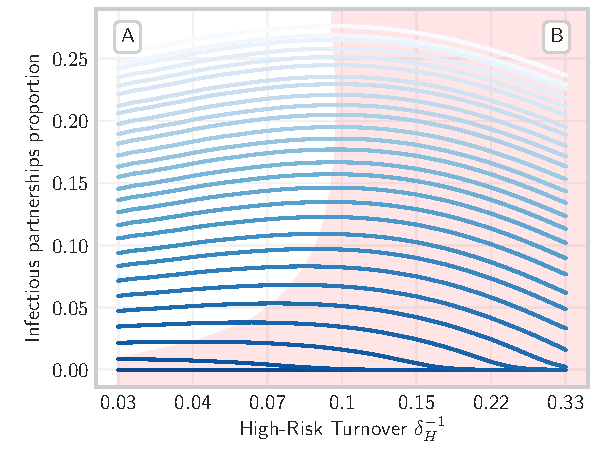
\includegraphics[width=\linewidth]{2d-XC-I}
    \caption{Proportion of available partnerships
      which are offered by infectious individuals $\bm{C}_{\mathcal{I}}$}
    \label{fig:2d-XC-I}
  \end{subfigure}
  \begin{subfigure}[t]{0.45\linewidth}
    \centering
    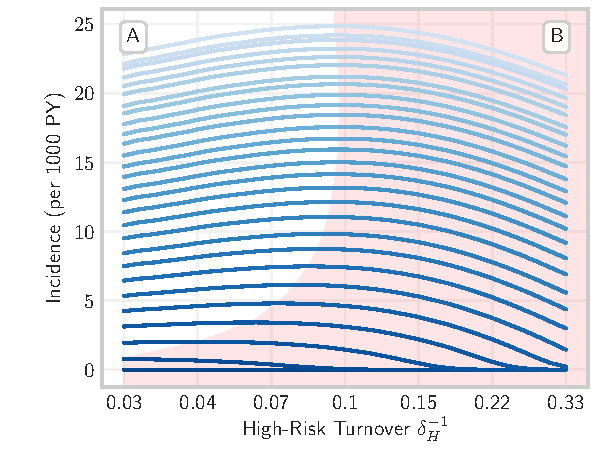
\includegraphics[width=\linewidth]{2d-incidence-all}
    \caption{Overall incidence $\lambda$}
    \label{fig:2d-incidence-all}
  \end{subfigure}
  \caption{Incidence and the dynamic factors of incidence versus turnover,
    for a range of treatment rates.
    Darker blue indicates higher treatment rate.
    The product of components (a) and (b) is proportional to
    (c) the proportion of total available contacts which are with infectious individuals
    and (d) overall incidence.}
  \label{fig:2d-incidence-factors}
\end{figure}
\par
Finally, Figure~\ref{fig:surface} summarizes trends in
overall equilibrium incidence and group-specific prevalence
with respect to both turnover $\phi$ and treatment rate $\tau$.%
\footnote{Figure~\ref{fig:surface-incidence-all}
  is the surface projection of the profiles shown in
  Figure~\ref{fig:2d-incidence-all}.}
Treatment consistently decreases equilibrium incidence (as noted above),
as well as prevalence, at all rates of turnover.
As suggested in Experiment 2.1, prevalence among the highest risk group
(Figure~\ref{fig:surface-prevalence-high})
also decreases with turnover for any rate of treatment.
Similarly, prevalence among the low risk group
(Figure~\ref{fig:surface-prevalence-low})
increases with turnover for moderate rates of turnover and treatment.
However, as turnover increases past the point which maximizes incidence,
prevalence among the low risk group peaks, and then declines.
As shown in Figure~\ref{fig:2d-incidence-factors},
the rate of turnover at which this occurs decreases with treatment rate.
Once again, trends in overall prevalence
roughly reflect those of the lowest risk group.
Finally, for high rates of treatment and/or turnover, the product of
the average contact rate of infectious individuals $\hat{C}_\mathcal{I}$
and the proportion of the population who are infected $\hat{\mathcal{I}}$
is too low to sustain the epidemic.
That is, the basic reproductive number $R_0$ declines to less than one,
and no epidemic is observed.%
\footnote{In fact, it can be shown that for extreme rates of turnover,
  a heterogeneous system (e.g. Full model) will converge on
  a homogeneous system (e.g. model V1).
  This result is shown in Figure~\ref{fig:hetero-converge}.}
\begin{figure}
  \centering
  \begin{subfigure}{0.45\linewidth}
    \centering
    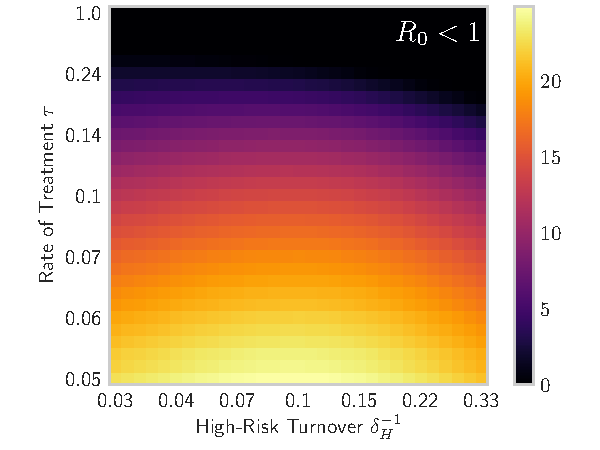
\includegraphics[width=\linewidth]{surface-incidence-all}
    \caption{Overall incidence}
    \label{fig:surface-incidence-all}
  \end{subfigure}
  \begin{subfigure}{0.45\linewidth}
    \centering
    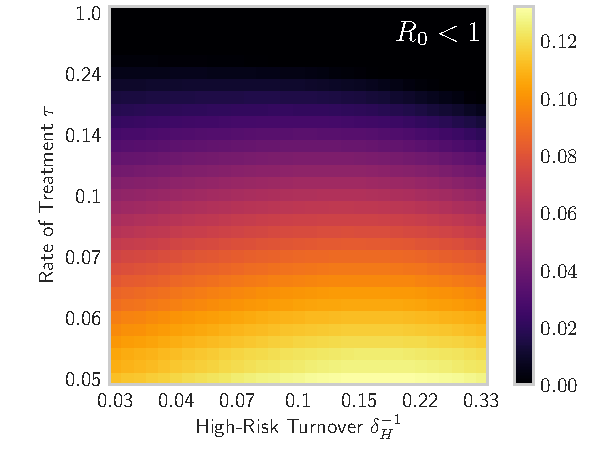
\includegraphics[width=\linewidth]{surface-prevalence-all}
    \caption{Overall prevalence}
    \label{fig:surface-prevalence-all}
  \end{subfigure}
  \begin{subfigure}{0.45\linewidth}
    \centering
    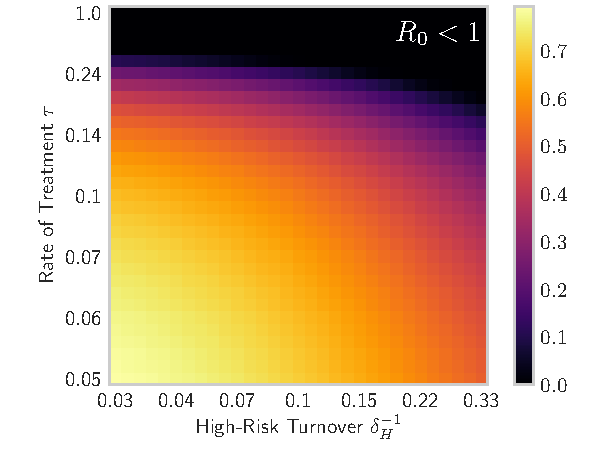
\includegraphics[width=\linewidth]{surface-prevalence-high}
    \caption{High risk prevalence}
    \label{fig:surface-prevalence-high}
  \end{subfigure}
  \begin{subfigure}{0.45\linewidth}
    \centering
    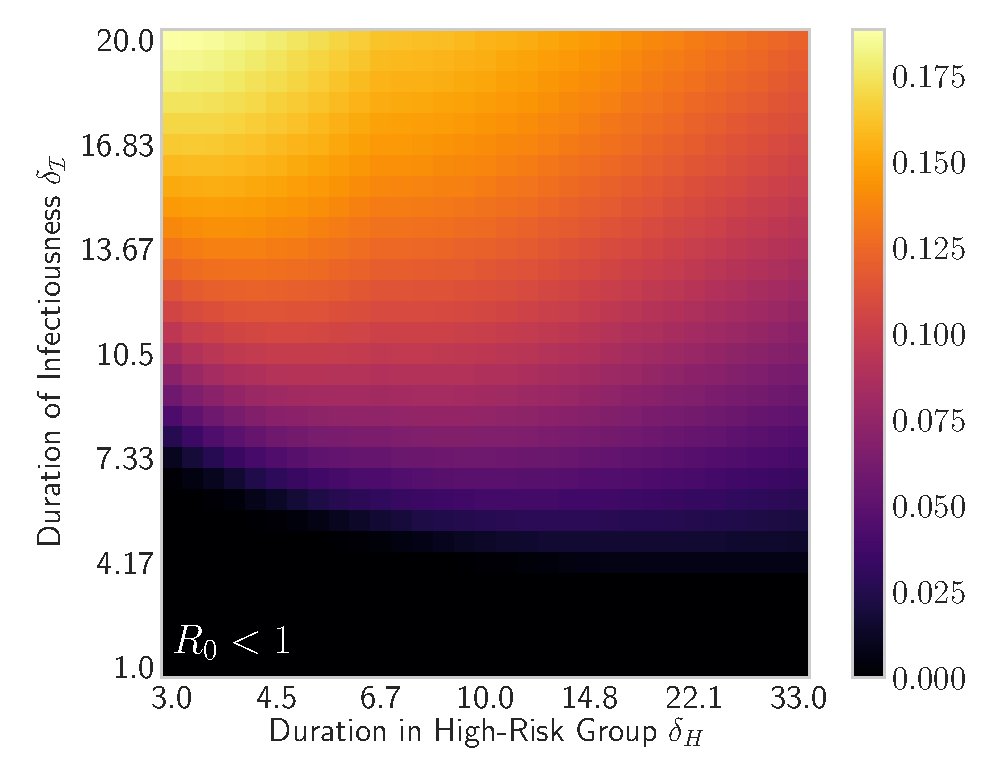
\includegraphics[width=\linewidth]{surface-prevalence-low}
    \caption{Low risk prevalence}
    \label{fig:surface-prevalence-low}
  \end{subfigure}
  \caption{Equilibrium prevalence and incidence for different rates of
    turnover $\phi$ (log scale) and
    treatment $\tau$ (log scale).}
  \label{fig:surface}
\end{figure}
% ==================================================================================================
\subsection{Fitted Models with Turnover}\label{ss:res-turnover-fit}
Finally, the influence of turnover on fitted models is explored.
For reference, the pre-calibration equilibrium prevalence predicted
among the and low high risk groups are shown in Figure~\ref{fig:tpaf-prevalence}.
The prevalence ratios are
$\input{\datapath/fit/Full-prevalence-ratio.txt}$ with turnover, and 
$\input{\datapath/fit/V3-prevalence-ratio.txt}$ without.
% --------------------------------------------------------------------------------------------------
\paragraph{Experiment 3.1: Inferred Risk Heterogeneity}
Following calibration of contact rates $C_H$~and~$C_L$,
both models predict an equilibrium prevalence 25\% and 5\%, as desired.
However, the fitted contact rates required to yield these outputs
are different with and without turnover (Table~\ref{tab:fitting});
the ratio of $C_H~/~C_L$ with turnover
($\input{\datapath/fit/Full-fit-C-ratio.txt}$)
is much higher than the ratio without turnover
($\input{\datapath/fit/V3-fit-C-ratio.txt}$).
Thus, for the model and conditions explored here,
the inferred heterogeneity in risk
is higher in the model with turnover than in the model without turnover.
This is because turnover acts to counteract the concentration of risk.
That is, in order to observe the same prevalence ratio in a system with turnover,
the ``risk homogenizing effects'' of turnover must be overcome by
greater heterogeneity in risk, as compared to a system without turnover.
\begin{table}
  \centering
  \caption{Equilibrium contact rates $C$ and prevalence $P$
    among the high $H$ and low $L$ risk groups
    predicted by the Full model (turnover) and V3 (no~turnover)
    before and after model fitting.}
  \label{tab:fitting}
  \begin{tabularx}{0.7\linewidth}{r *{6}{Y}}
	\toprule
  Model & $C_H$ & $C_L$ & $C_H~/~C_L$ & $P_H$ & $P_L$ & $P_H~/~P_L$\\\midrule
  Base &
    \input{\datapath/fit/Base-C-high.txt}
  & \input{\datapath/fit/Base-C-low.txt}
  & \input{\datapath/fit/Base-C-ratio.txt}
  & \input{\datapath/fit/Base-prevalence-high.txt}
  & \input{\datapath/fit/Base-prevalence-low.txt}
  & \textbf{\input{\datapath/fit/Base-prevalence-ratio.txt}}\\
  V3 &
    \input{\datapath/fit/V3-C-high.txt}
  & \input{\datapath/fit/V3-C-low.txt}
  & \input{\datapath/fit/V3-C-ratio.txt}
  & \input{\datapath/fit/V3-prevalence-high.txt}
  & \input{\datapath/fit/V3-prevalence-low.txt}
  & \textbf{\input{\datapath/fit/V3-prevalence-ratio.txt}}\\
  Base [fit] &
    \input{\datapath/fit/Base-fit-C-high.txt}
  & \input{\datapath/fit/Base-fit-C-low.txt}
  & \textbf{\input{\datapath/fit/Base-fit-C-ratio.txt}}
  & \input{\datapath/fit/Base-fit-prevalence-high.txt}
  & \input{\datapath/fit/Base-fit-prevalence-low.txt}
  & \input{\datapath/fit/Base-fit-prevalence-ratio.txt}\\
  V3 [fit] &
    \input{\datapath/fit/V3-fit-C-high.txt}
  & \input{\datapath/fit/V3-fit-C-low.txt}
  & \textbf{\input{\datapath/fit/V3-fit-C-ratio.txt}}
  & \input{\datapath/fit/V3-fit-prevalence-high.txt}
  & \input{\datapath/fit/V3-fit-prevalence-low.txt}
  & \input{\datapath/fit/V3-fit-prevalence-ratio.txt}\\
  \bottomrule
\end{tabularx}
\end{table}
% --------------------------------------------------------------------------------------------------
\paragraph{Experiment 3.2: TPAF of the High Risk Group}
Figure~\ref{fig:tpaf} shows the estimated TPAF of the high risk group
with and without turnover, and before and after model fitting.
The TPAF approaches 1.0 for all models over a 100 year time horizon,
indicating that unmet treatment needs of the high risk group
are central to epidemic persistence in all models.
Additionally, no TPAFs intersect during this period,
so relative differences between TPAFs by model can be described irrespective of time horizon.
\par
Before model fitting (Figure~\ref{fig:tpaf}, solid lines),
the model without turnover estimates a larger TPAF of the high risk group
than the model with turnover.
This can be attributed to the larger equilibrium prevalence ratio before model fitting
(Table~\ref{tab:fitting}, Figure~\ref{fig:tpaf-prevalence}),
which results in more onward transmission from the high prevalence high risk group.
In other words, the importance of reaching the high risk group
in a context without turnover is higher than in a context with turnover.
\par
However, after fitting contact rates $C_H$~and~$C_L$ to
high and low risk prevalence targets as described above,
the model with turnover estimates a higher TPAF of the high risk group
than the model without turnover
(Figure~\ref{fig:tpaf}, dashed lines).
This reversal in which model predicts a higher TPAF can be explained by two factors.
First, the equilibrium prevalence ratios predicted by the models with and without turnover
are equalized through model fitting to the same targets.
As a result, higher prevalence among the high risk group in the model without turnover
no longer contributes to an increased TPAF estimate by this model.
Second, as shown in Experiment 3.1, 
the ratio of fitted contact rates $C_H~/~C_L$ in the model with turnover
are higher than in the model without.
This affords a higher risk of onward transmission to the high risk group
in the model with turnover, and thus an increased TPAF.
This result then implies that
models which fail to capture turnover dynamics which are truly present in reality
may underestimate the TPAF of high risk groups.
Consequently, the importance of prioritizing high risk groups
to achieve epidemic control may be similarly underestimated by such models.
\begin{figure}
  \centering
  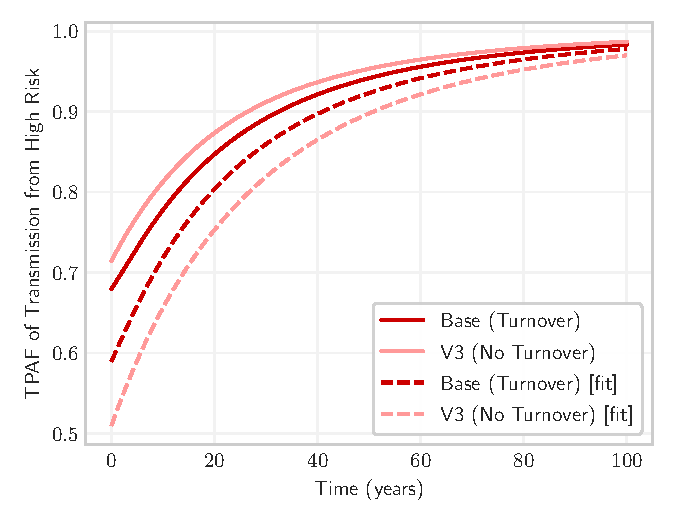
\includegraphics[width=0.6\linewidth]{tpaf-tpaf-high-all}
  \caption{Transmission population attributable fraction (TPAF-from)
    of the high risk group with and without turnover,
    and with and without fitted contact rates to group-specific prevalence.}
  \label{fig:tpaf}
\end{figure}
%% SS: This section perhaps could be a bit clearer as clearly very important
%% Is there a way to more explicitly talk about new infections
%% in the low / medium risks coming from prevalent infections
%% entering into these states from high risk groups and that
%% subsequent infections emanating from these individuals are thus still
%% linked back to prior history in the high risk group? 